\listfiles
\documentclass[%
 reprint,%
%secnumarabic,%
 amssymb, amsmath,%
 aip,cha,%
%groupedaddress,%
%frontmatterverbose,
]{revtex4-1}

\usepackage{docs}%
\usepackage{bm}%
\usepackage{mathtools}
\usepackage{graphicx}
\usepackage{tikz}
\usepackage[colorlinks=true,linkcolor=blue]{hyperref}%
%\nofiles
\expandafter\ifx\csname package@font\endcsname\relax\else
 \expandafter\expandafter
 \expandafter\usepackage
 \expandafter\expandafter
 \expandafter{\csname package@font\endcsname}%
\fi
%\hyphenation{title}

\begin{document}

\title{Streak Camera System and Tune Resonance Tool}%

\author{L. Dovlatyan, M. Ries, P. Goslawski, and friends at HZB}%
\email{levondov@berkeley.edu}
\affiliation{University of California Berkeley,94720 Berkeley, CA, USA}%

\date{August 2014}%
%\revised{August 2010}%

\maketitle

\tableofcontents

\section{Introduction}

The Helmholtz-Zentrum Berlin is a facility that operates two synchrotron light sources: BESSY II and the MLS. One of the long term goals of this center is to continually make bunch lengths as short as possible in storage rings. The current bunch length $\sigma_0$ is defined by longitudinal dynamics as
\begin{equation}
\sigma_0 = \delta_o \sqrt{\frac{E_0}{f_0} \frac{\alpha}{eU^\prime}}
\end{equation}
and can be changed for a given machine with defined energy spread $\delta_0$, energy $E_0$ and revolution frequency $f_0$ by changing the momentum compaction factor $\alpha$ or the cavity voltage $U^\prime$ which is defined as $U^\prime = 2\pi f_{rf} U_0$.

A way to go about this is through lattice design by changing the momentum compaction factor. An important part of lattice design involves picking a good working point to avoid the tune resonances of the machine. A tune resonance program was therefore developed which can be used to view the current working point and resonance lines given only a few input parameters from the EPICS control systems.

Diagnostic tools are needed in order to investigate shortest bunches in storage rings. A new streak camera was recently purchased for the MLS, and is currently being setup and tested. The Metrology Light Source (MLS) is an electron storage ring designed as a dedicated UV and VUV source; it has an asymmetric double-bend achromate design as well as six beamlines, two of which are located on a second floor, above the synchrotron. Both the new and the old streak cameras are setup with a UV beamline on the second floor, directly above the machine. Being on the second floor and having the cameras setup far away from the beamline required advanced optical paths in order to get a focused beam into the slits of the cameras.

\section{Tune Resonance Program\cite{Note1}}

The program is based on the principal of optical resonances. Different magnets have different order magnetic fields and can effect the betatron oscillations in the horizontal and vertical planes. For example, a quadrupole magnetic field can produce a second order betatron oscillation resonance. 
\begin{table}[h]
\centering
\begin{tabular}{l|r}
driving field & condition \\
\hline
\hline
dipole & $Q = p$ \\
quadrupole & $2Q = p$ \\
sextupole & $3Q = p$ \\
octupole & $4Q = p$ \\
npole & $nQ = p$\\
\end{tabular}
\caption{\label{tunetable}Driving fields and corresponding resonance conditions that must be met.}
\end{table}
$p$ from table I means the $p$th harmonic of the function $ \beta^{3/2} (s) g^\prime (s) $ where $ \beta (s)$ is the beta or amplitude function and $g (s)$ is directly proportional to the field errors of the magnetics.

Because of the coupling of the betatron oscillations in different planes, certain optical resonance conditions must be satisfied by the following equation:
\begin{equation}
 m \; Q_x + n \; Q_y = p
\end{equation}
Where $m$,$n$, and $p$ are integer values. $Q_x$ and $Q_y$ are the horizontal and vertical positions of the tune. The sum of $ |m| + |n| $ is called the order of the resonances. For stable operation $Q_x$ and $Q_y$ must be chosen to be far away from any optical resonances. This program helps tackle this problem by providing a visual guide and a simple GUI to aid the operator in picking an adequate working point for the machine.
\subsection{Developement}
The program is written in Python and completely open source. This provided the opportunity to integrate with EPICS (Experimental Physics and Industrial Control System) through a special python package called PyEpics and build a GUI system using wxPython to make the program simple to use. Much of the program also relies heavily on numpy and matplotlib packages available for Python.

The biggest feature of the program is a 'live mode' option that is able to give the current tune position numerically and graphically. Using the proper epics channels, the program is able to grab the four values it needs to calculate the non integer tune: the RF cavity frequency $f_{rf}$, the harmonic number $h$, and the horizontal and vertical betatron oscillation frequencies $f_x,f_y$. The program can check and update the tune several times a second, but in order to have the visual display updated, a threading process was used to avoid having the GUI freeze up while in live mode. The threading process is able to do all the processing and updating of the matplotlib graph, continously updating the working point on the plot.

\subsection{Customizability}
Various customizability options are available for the program. Changing color settings, removing certain resonance lines, and adjusting for mirrored tunes are just some features available for the user. Being able to display phase advance resonance lines is another unique feature included in the program.

Aside from accelerators having to position their working points away from resonane lines, they must also consider the phase advanced resonance lines as these are much more powerful and dangerous to approach with a working point. Given the number of unit cells for the machine, the program is able to display a tune diagram with the phase advance resonance lines along with the working points. This feature can complement the live mode option available with the program. If an operator wants to move the working point and cross resonance lines, the program can be used as a visual guide in order to avoid the phase advanced resonance lines (colored in red in figure~\ref{fig1}) which will more than likely kill the beam.
\begin{figure}[htb]
\begin{center}
\includegraphics[width=200pt]{image.pdf}
\caption{Tune resonance diagram displaying phase advance lines (4 unit cells) for the MLS}
\label{fig1}
\end{center}
\end{figure}

\subsection{Future Improvements}
The program's availability on github\cite{Note1} allows for updates and improvements to be added in the future. Because of a lack of time, some improvements and features will be added at a later date. One of these improvements is the amount of CPU power the program uses when running in live mode. The problem stems from the matplotlib package having to constantly update the graph/plot several times a second; this process ends up consuming a lot of CPU power and eventually slows down the program significantly. Aside from this, there are minor improvements that will be added in occasionally depending on the amount of free time available.

\section{Streak Camera for Bunch Length Measurements}
A streak camera is a device used to take pictures of very fast light phenomena. The resulting images however are not like that of a typical camera, but instead are given in a plot of intensity vs time vs position.
\begin{figure}[htb]
\begin{center}
\includegraphics[width=250pt]{streakdiagram.pdf}
\caption{Streak camera operational principals\cite{Note2}}
\label{streakdiagram}
\end{center}
\end{figure}

How the camera actually works is illustrated in figure 3. Radiation enters the camera's slit as photons with varying intensity emitted from the electrons in the beam; it then goes through some lens before hitting a photocathode. The photocathode converts the photons into a certain number of electrons proportional to the intensity of the light. The accelerating mesh then accelerates the electrons towards the phosphor screen. The electrons then go through a sweeping electric field that deflects them at slightly different angles vertically depending on the arrival time of the electrons. Additionally, a horizontal sweep might be switched on and used to get multi bunch measurements. The micro channel plate then multiplies the electrons several thousand times in order for their impact on the phosphor screen to be detectable. Finally, the electrons hit the phosphor screen and are transformed back into photons; their positions on the screen depend on their arrival time at the sweeping electrode. The earliest electrons are deflected to the top of the screen and the latest electrons are at the bottom of the screen; this turns the vertical axis into a time axis and allows the measuring of the bunch length for the beam either with FWHM or sigma.
\begin{figure}
\begin{center}
\includegraphics[width=200pt]{uplot.pdf}
\caption{Undulator Radiation from U125 at the MLS between the range of 15 to 35 nm}
\label{Uradiation}
\end{center}
\end{figure}

\subsection{Setup\cite{Note3}}
The setup of the streak cameras proved to be quite a challenge. The cameras had to be on top of a specific optical table that was positioned behind and above the beamline; this required an optical path that would provide six degrees of freedom.
\begin{figure}[htb]
\begin{center}
\includegraphics[width=250pt]{diagramtext.pdf}
\caption{Rough diagram of stream camera setup}
\label{diagram}
\end{center}
\end{figure}

The very first thing done when setting up the optical paths was to align a helium neon laser with the beam using a splitter. Beamtime at a synchrotron is expensive and not always available, but having a laser that is perfectly aligned with the beam allowed us to continue setting up the optical paths using the laser instead of the beam. The first piece along the optical path is a bandpass filter lens which allows wavelengths between 630 and 640 nm; this is also the wavelength range of the laser. However, in order to have the synchrotron and undulator radiation pass through this filter, the undulator gap must be optimized by shifting the intensities to fit in the range of our filter. Figure~\ref{Uradiation} shows a plot of the undulator radiation for the undulator at the MLS (U125). Next we pass through an aperture that is used to help focus the beam before finally hitting a plane mirror at the top of our vertical beam.

Looking at the coherence condition for undulator radiation, 
\begin{equation}
\lambda_w = \frac{\lambda_u}{2\gamma^2} (1 + \frac{K^2}{2} + \gamma^2\Theta_0^2)
\end{equation}
there are a few variables that can be changed in order to shift the wavelengths of the radiation. Changing the undulator period $\lambda_u$ or the laboratory frame angle $\Theta_0$ is not really an option. This leaves the beam energy $\gamma$ and the undulator parameter $K$. For our purposes the undulator parameter was the easiest to manipulate.
\begin{equation}
K = \frac{e B \lambda_u}{2\pi m_e c}
\end{equation}
The undulator parameter $K$ is directly proportional to the on axis magnetic field $B$. By changing the undulator gapping we were able to manipulate this magnetic field resulting in the shifiting of the wavelengths of the radiation into the range of our filter.

The next thing we did is setup the horizontal optical table. An ideal setup
\begin{figure}[htb]
\begin{center}
\fbox{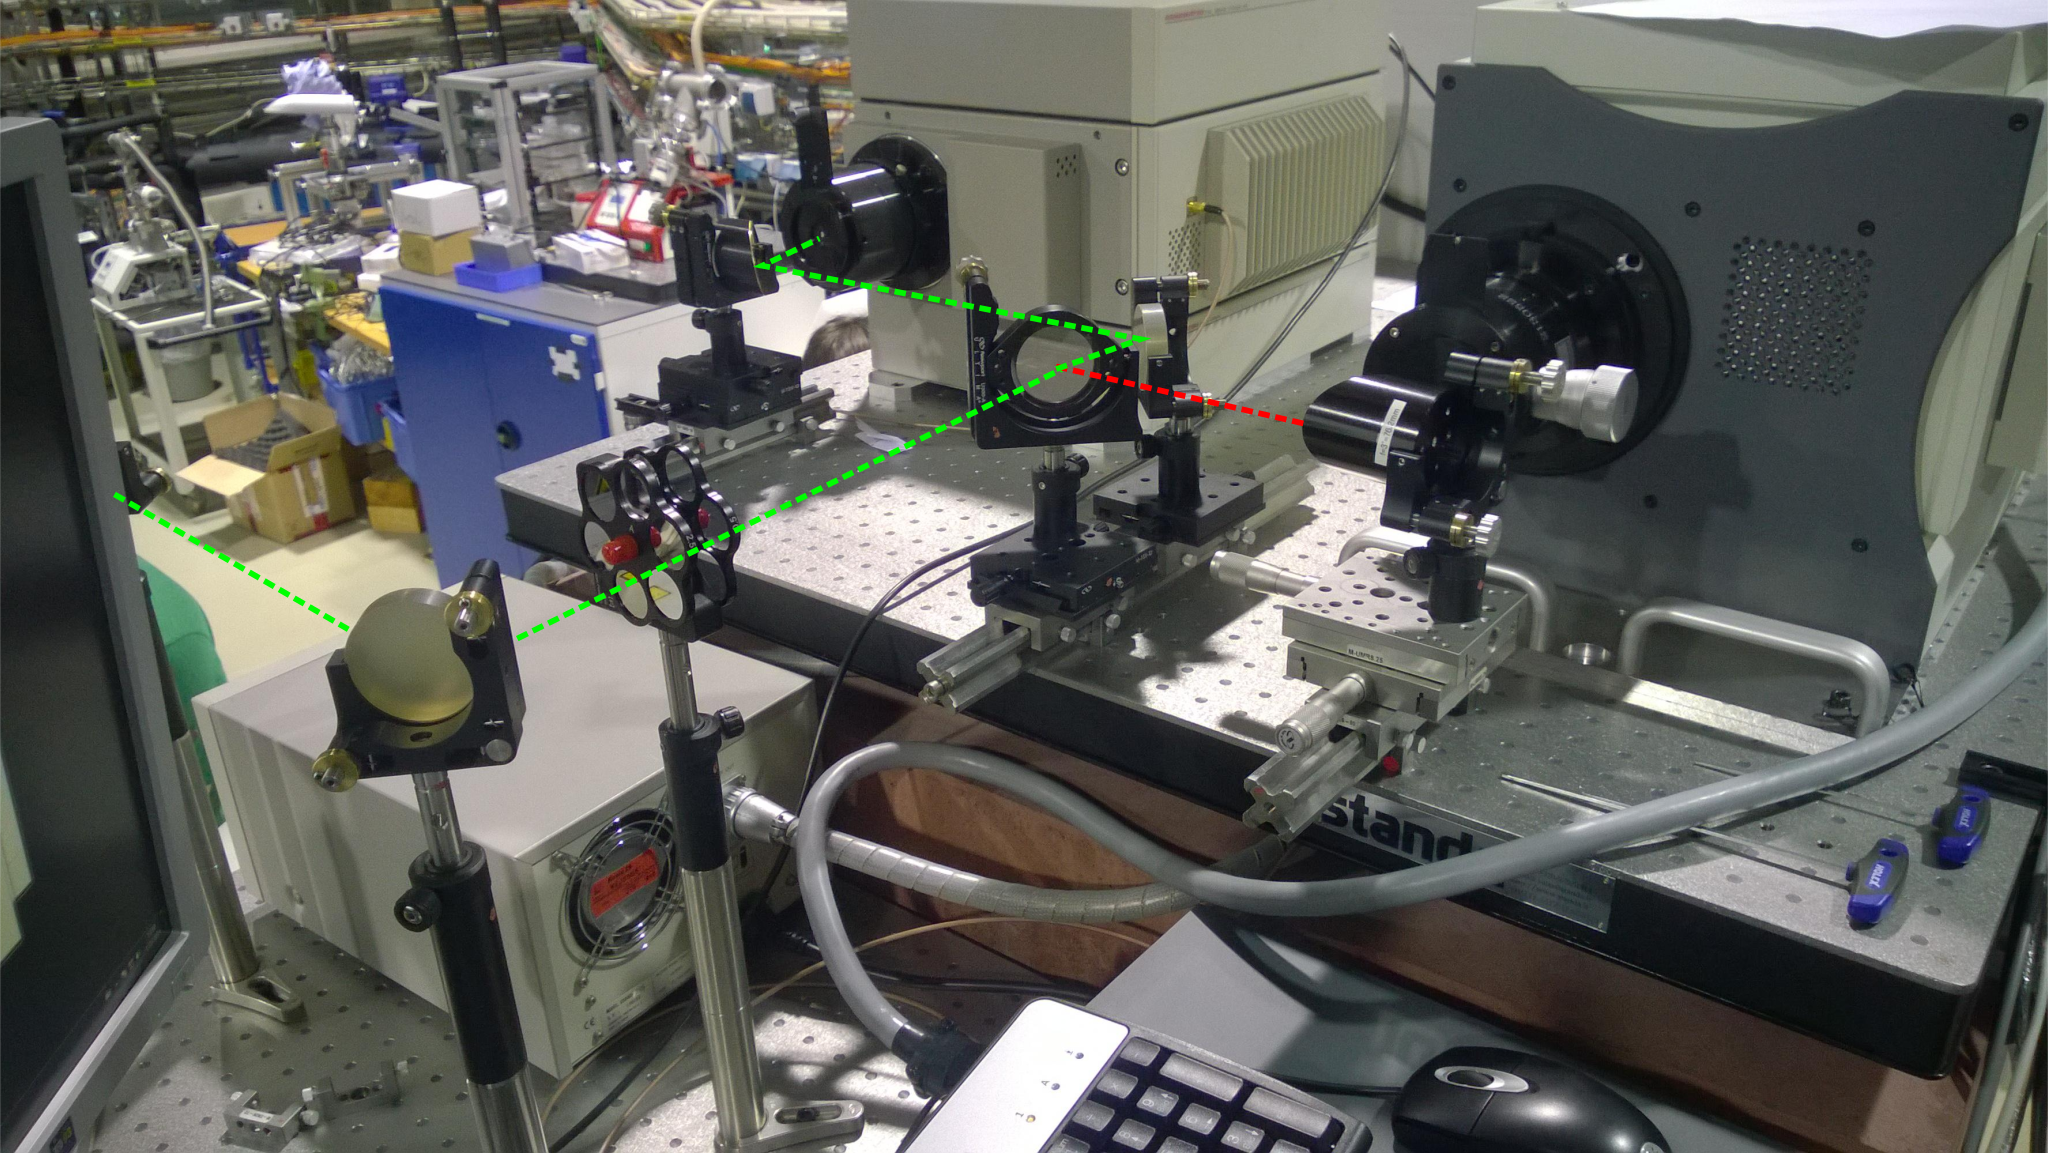
\includegraphics[width=175pt]{horizontaltable.pdf}} \\[0.5cm]
\caption{Horizontal optical table setup}
\label{hortable}
\end{center}
\end{figure}
that allowed dual streak camera operation was constructed. Continuing with the beam path after the vertical beam, we pass through a few plane mirrors before hitting another filter. The new streak camera's cathode was a lot more sensitive than the old camera's, and as a result, the beam's intensity needed to be lowered in order to avoid burning out the cathode; this was accomplished with a filter wheel placed along the optical path which can be easily adjusted to find the right intensity. 

After the filter wheel, the last part of the optical path is reached. A splitter and plane mirror are used to split and redirect the beam in two different directions. One path continues to the new streak camera while another splits off and heads towards the old camera. Finally, a pair of toroidal mirrors placed right before both cameras are used to focus the beam into the slits of both cameras.

\subsection{Operation}

Initial measurements with the new streak were taken at the MLS\cite{Note4}. A single bunch measurement is shown in figure 6 along with an intensity vs time plot. Fitting a normal gaussian to the plot and finding a corresponding sigma value can give us the electron bunch length.
\begin{figure}[htb]
\begin{center}
\begin{tikzpicture}
\node at (0,0) {\includegraphics[width=250pt]{lowalpha_1uA.pdf}};
\node at (0,0) {\includegraphics[width=250pt]{lowalpha_1uAgraph.pdf}};
\end{tikzpicture}
\caption{single bunch measurement in low alpha mode at the MLS}
\label{measurement}
\end{center}
\end{figure}

\subsection{Future Improvements}
There is still much to be done with the streak camera. One major problem that was not fully resolved is getting both vertical and horizontal focal points of the beam into the streak camera pin hole. Because the beamline is on the second floor, at some point a mirror was used to deflect the beam upstairs; this mirror caused the horizontal and vertical focal points of the beam to diverge from each other. The focal points are a few centimeters apart which causes problems when trying to get the beam aligned properly. Two options are available to try and fix this problem. A custom toroidal like mirror can be ordered that can focus both beams back into one spot, or two normal toroidal mirrors positioned right after each other can be used to align the focal points correctly. The latter seems like a much more reasonable solution to the problem.

Having a lab view system to control all the values and parameters from the steak camera software would also be a much needed improvement. Along with this lab view system, one can put in safety measures to help prevent the camera from breaking. Because the camera is so sensitive to the beam and can easily have its cathode burned, a remote program controlling the filter and shutter systems will help prevent any expensive accidents from occuring.

\section{Conclusion and acknowledgements}
Both the tune resonance program and the steak camera setup ended up teaching me a tremendous amount not only in the field of accelerator physics, but also in optical path designs, programming with python and related packages, and learning about poster design with LaTex. The tune resonance program will continue to be supported and updated by me as much as time allows and at the request of others.

I would like to thank Markus and Paul as well as everyone else in the accelerator group at HZB for mentoring, teaching, and guiding me through the last couple weeks. It has been an amazing experience to spend the summer here in Berlin and it will always be remembered.


\begin{thebibliography}{9}\label{sec:TeXbooks}%
\bibitem{Note1}
Source code can be found on the following github page: 
\url{https://github.com/levondov/TuneResonancePython}.
%
\bibitem{Note2}
Hamamatsu,
\emph{Guide to Streak Cameras}
(HAMAMATSU PHOTONICS K.K., Hamamatsu City, Japan, 2008)
\url{http://www.hamamatsu.com/resources/pdf/sys/e_streakh.pdf}.
%
\bibitem{Note3} 
More pictures of the optical path setup can be found here:
\url{http://1drv.ms/1oCjkjI}
%
\bibitem{Note4} 
To Find more images of the streak camera measurements, see here:
\url{https://github.com/levondov/PosterTex/tree/master/IP}
%
\bibitem[Knuth(1986)]{TeXbook} 
D. E. Knuth, 
\emph{The \TeX book} 
(Addison-Wesley, Reading, MA, 1986). 

\end{thebibliography}

\end{document}

